\documentclass[12pt,twocolumn,twoside,lineno]{gsajnl}
% Use the documentclass option 'lineno' to view line numbers

\usepackage{epstopdf}

\articletype{gs} % article type
% {inv} Investigation
% {gs} Genomic Selection
% {goi} Genetics of Immunity
% {gos} Genetics of Sex
% {mp} Multiparental Populations

\runningtitle{GENETICS Journal Template on Overleaf} % For use in the footer
\runningauthor{FirstAuthorLastname \textit{et al.}}

\title{Template for preparing your submission to \textit{GENETICS} using Overleaf}

\author[1,$\dagger$]{Author One}
\author[1]{Author Two}
\author[2]{Author Three}
\author[2,3]{Author Four}
\author[4,$\ast$]{Author Five}

\affil[1]{Author one affiliation}
\affil[2]{Author two affiliation}
\affil[3]{Author three affiliation}
\affil[4]{Author four affiliation}
\affil[$\dagger$]{These authors contributed equally to this work.}

% Use the \equalcontrib command to mark authors with equal
% contributions, using the relevant superscript numbers
%\equalcontrib{1}
%\equalcontrib{2}

\correspondingauthoraffiliation[$\ast$]{Corresponding author: Please insert the affiliation correspondence address and email for the corresponding author. The corresponding author should be marked with the relevant number in the author list, as shown in the example.}

\begin{abstract}
The abstract should be written for people who may not read the entire paper, so it must stand on its own. The impression it makes usually determines whether the reader will go on to read the article, so the abstract must be engaging, clear, and concise. In addition, the abstract may be the only part of the article that is indexed in databases, so it must accurately reflect the content of the article. A well-written abstract is the  most effective way to reach intended readers, leading to more robust search, retrieval, and usage of the article.

Please see additional guidelines notes on preparing your abstract below.
\end{abstract}

\keywords{Keyword; Keyword2; Keyword3}

\dates{\rec{xx xx, xxxx} \acc{xx xx, xxxx}}

\begin{document}

\maketitle
\thispagestyle{firststyle}
%\slugnote
%\firstpagefootnote
\vspace{-13pt}% Only used for adjusting extra space in the left column of the first page

\lettrine[lines=2]{\color{color2}T}{}his \textit{Genetics} journal template is provided to help you write your work in the correct journal format. Instructions for use are provided below. Note that by default line numbers are present to aid reviewers and editors in reading and commenting on your manuscript. To remove line numbers, remove the \texttt{lineno} option from the \verb|\documentclass| declaration.
\section{Your abstract}

In addition to the guidelines provided in the example abstract above, your abstract should:

\begin{itemize}
\item provide a synopsis of the entire article;
\item begin with the broad context of the study, followed by specific background for the study;
\item describe the purpose, methods and procedures, core findings and results, and conclusions of the study;
\item emphasize new or important aspects of the research;
\item engage the broad readership of GENETICS and be understandable to a diverse audience (avoid using jargon);
\item be a single paragraph of less than 250 words;
\item contain the full name of the organism studied;
\item NOT contain citations or abbreviations.
\end{itemize}

\section{Introduction}

Authors should be mindful of the broad readership of the journal and set the stage for the importance of the work to a generalist reader. The scope and impact of the work should be clearly stated.

In individual organisms where a mutant is being studied, the rationale for the study of that mutant must be clear to a geneticist not studying that particular organism. Similarly, study of particular phenotypes should be justified broadly and not on the basis of interest for that organism alone. General background on the importance of the genetic pathway and/or phenotype should be provided in a single, well-reasoned paragraph near the beginning of the introduction.

\section{Materials and methods}
\label{sec:materials:methods}

Manuscripts submitted to GENETICS should contain a clear description of the experimental design in sufficient detail so that the experimental analysis could be repeated by another scientist. If the level of detail necessary to explain the protocol goes beyond two paragraphs, give a short description in the main body of the paper and prepare a detailed description for supporting information.  For example, details would include indicating how many individuals were used, and if applicable how individuals or groups were combined for analysis. If working with mutants indicate how many independent mutants were isolated. If working with populations indicate how samples were collected and whether they were random with respect to the target population.


\subsection{Statistical analysis}

Indicate what statistical analysis has been performed; not just the name of the software and options selected, but the method and model applied. In the case of many genes being examined simultaneously, or many phenotypes, a multiple comparison correction should be used to control the type I error rate, or a rationale for not applying a correction must be provided. The type of correction applied should be clearly stated. It should also be clear whether the p-values reported are raw, or after correction. Corrected p-values are often appropriate, but raw p-values should be available in the supporting materials so that others may perform their own corrections. In large scale data exploration studies (e.g. genome wide expression studies) a clear and complete description of the replication structure must be provided.

\section{Results}

The results and discussion should not be repetitive and give a factual presentation of the data with all tables and figures referenced. The discussion should not summarize the results but provide an interpretation of the results, and should clearly delineate between the findings of the particular study and the possible impact of those findings in a larger context. Authors are encouraged to cite recent work relevant to their interpretations. Present and discuss results only once, not in both the Results and Discussion sections. It is acceptable to combine results and discussion in order to be succinct.

\section{Discussion}

\subsection{Numbers} In the text, write out numbers nine or less except as part of a date, a fraction or decimal, a percentage, or a unit of measurement. Use Arabic numbers for those larger than nine, except as the first word of a sentence; however, try to avoid starting a sentence with such a number.

\subsection{Units} Use abbreviations of the customary units of measurement only when they are preceded by a number: "3 min" but "several minutes". Write "percent" as one word, except when used with a number: "several percent" but "75\%." To indicate temperature in centigrade, use ° (for example, 37°); include a letter after the degree symbol only when some other scale is intended (for example, 45°K).

\subsection{Nomenclature and italicization} Italicize names of organisms even when  when the species is not indicated.  Italicize the first three letters of the names of restriction enzyme cleavage sites, as in HindIII. Write the names of strains in roman except when incorporating specific genotypic designations. Italicize genotype names and symbols, including all components of alleles, but not when the name of a gene is the same as the name of an enzyme. Do not use "+" to indicate wild type. Carefully distinguish between genotype (italicized) and phenotype (not italicized) in both the writing and the symbolism.

\subsection{Cross references}
Use the \verb|\nameref| command with the \verb|\label| command to insert cross-references to section headings. For example, a \verb|\label| has been defined in the section \nameref{sec:materials:methods}.

\section{Conclusion}

Add citations using the \verb|\citep{}| command, for example \citep{neher2013genealogies} or for multiple citations, \citep{neher2013genealogies, rodelsperger2014characterization,Falush16}  \citep{neher2013genealogies}

\section{Figures and tables}

Figures and Tables should be labelled and referenced in the standard way using the \verb|\label{}| and \verb|\ref{}| commands.

\subsection{Sample figure}

Figure \ref{fig:spectrum} shows an example figure.

\begin{figure}[t]
\centering
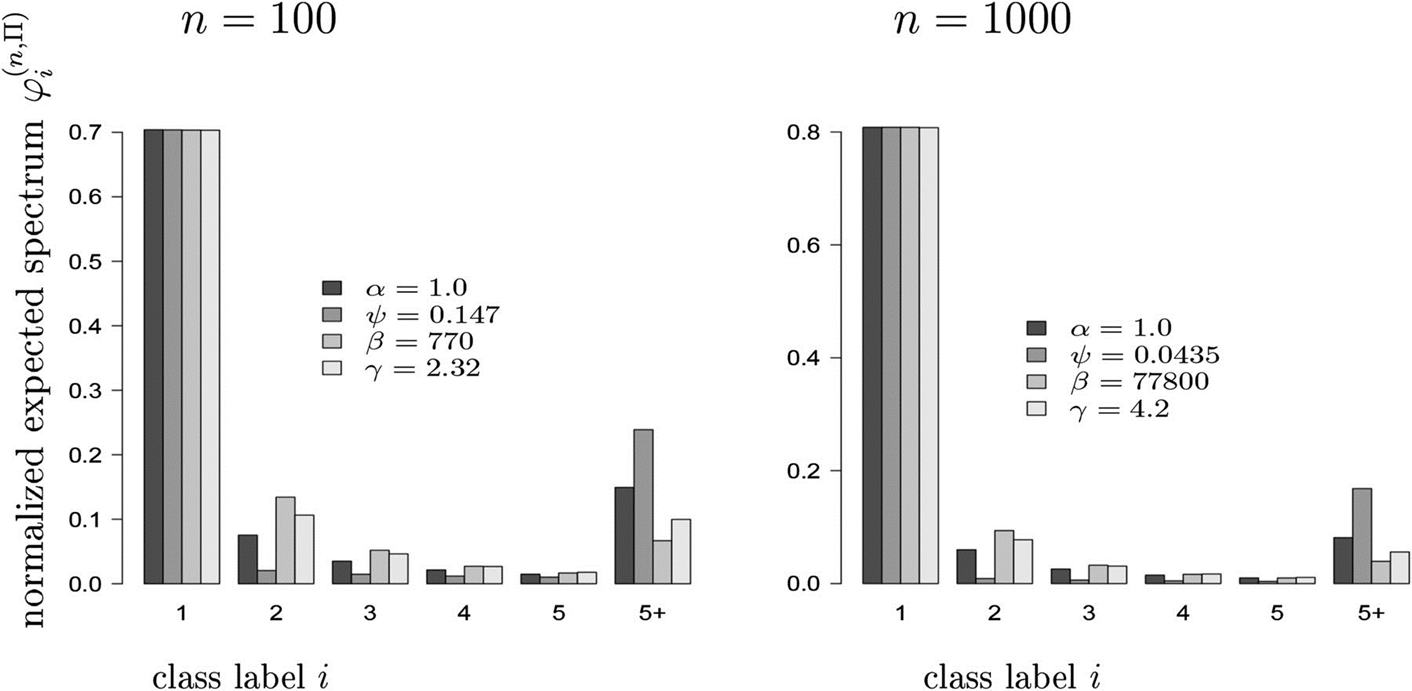
\includegraphics[width=\linewidth]{example-figure}
\caption{Example figure from \url{10.1534/genetics.114.173807}. Please include your figures in the manuscript for the review process. You can upload figures to Overleaf via the Project menu. Images of photographs or paintings can be provided as raster images. Common examples of raster images are .tif/.tiff, .raw, .gif, and .bmp file types. The resolution of raster files is measured by the number of dots or pixels in a given area, referred to as “dpi” or “ppi.”
\begin{itemize}
\item  minimum resolution required for printed images or pictures: 350dpi
\item  minimum resolution for printed line art: 600dpi (complex or finely drawn line art should be 1200dpi)
\item minimum resolution for electronic images (i.e., for on-screen viewing): 72dpi
\protect\end{itemize}
Images of maps, charts, graphs, and diagrams are best rendered digitally as geometric forms called vector graphics. Common file types are .eps, .ai, and .pdf. Vector images use mathematical relationships between points and the lines connecting them to describe an image. These file types do not use pixels; therefore resolution does not apply to vector images.
Label multiple figure parts with A, B, etc. in bolded. Legends should start with a brief title and should be a self-contained description of the content of the figure that provides enough detail to fully understand the data presented. All conventional symbols used to indicate figure data points are available for typesetting; unconventional symbols should not be used. Italicize all mathematical variables (both in the figure legend and figure) , genotypes, and additional symbols that are normally italicized.}%
\label{fig:spectrum}
\end{figure}

\begin{figure}[htbp]
\centering
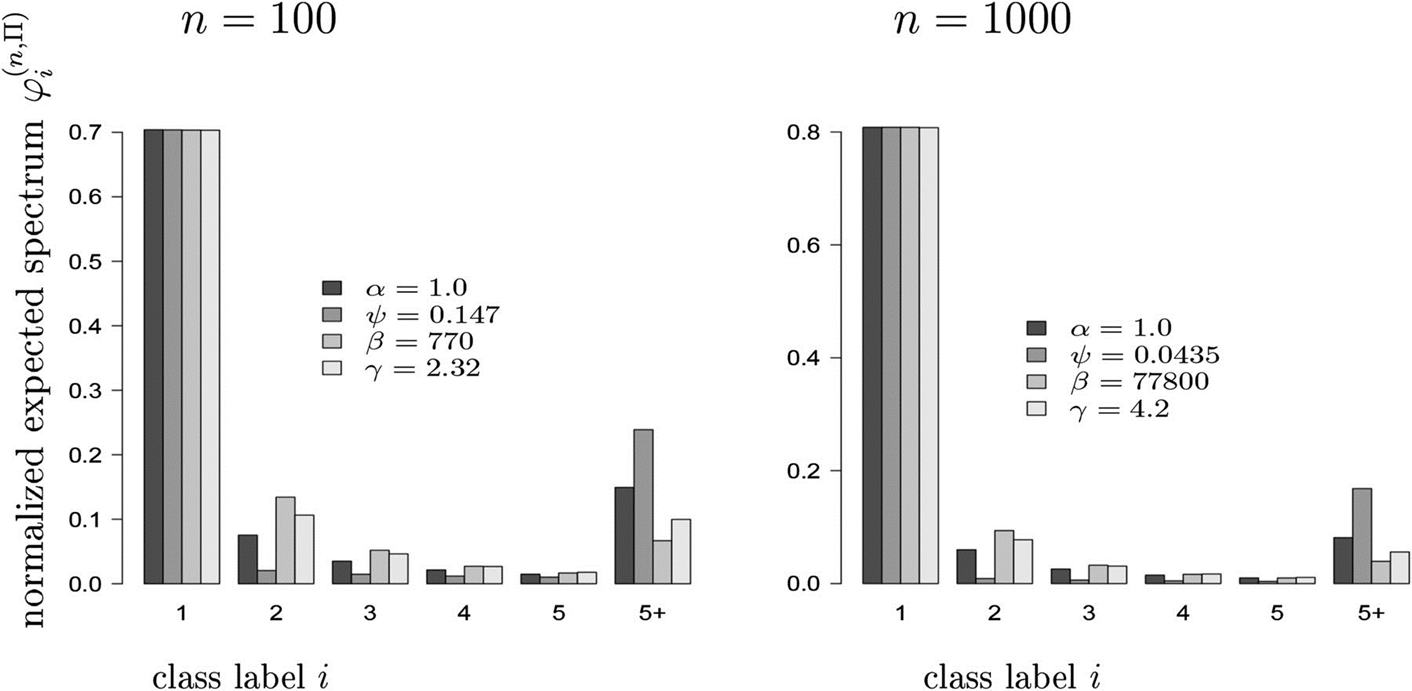
\includegraphics[width=\linewidth]{example-figure}
\caption{Example movie (the figure file above is used as a placeholder for this example). \textit{GENETICS} supports video and movie files that can be linked from any portion of the article - including the abstract. Acceptable formats include .asf, avi, .wav, and all types of Windows Media files.
}%
\label{video:spectrum}
\end{figure}

\subsection{Sample table}

Table \ref{tab:shape-functions} shows an example table. Avoid shading, color type, line drawings, graphics, or other illustrations within tables. Use tables for data only; present drawings, graphics, and illustrations as separate figures. Histograms should not be used to present data that can be captured easily in text or small tables, as they take up much more space.

Tables numbers are given in Arabic numerals. Tables should not be numbered 1A, 1B, etc., but if necessary, interior parts of the table can be labeled A, B, etc. for easy reference in the text.

\section{Sample equation}

Let $X_1, X_2, \ldots, X_n$ be a sequence of independent and identically distributed random variables with $\text{E}[X_i] = \mu$ and $\text{Var}[X_i] = \sigma^2 < \infty$, and let
\begin{equation}
S_n = \frac{X_1 + X_2 + \cdots + X_n}{n}
      = \frac{1}{n}\sum_{i}^{n} X_i
\label{eq:refname1}
\end{equation}
denote their mean. Then as $n$ approaches infinity, the random variables $\sqrt{n}(S_n - \mu)$ converge in distribution to a normal $\mathcal{N}(0, \sigma^2)$.

\section{Data availability}

The inclusion of a Data Availability Statement is a requirement for articles published in GENETICS. Data Availability Statements provide a standardized format for readers to understand the availability of data underlying the research results described in the article. The statement may refer to original data generated in the course of the study or to third-party data analyzed in the article. The statement should describe and provide means of access, where possible, by linking to the data or providing the required unique identifier.

For example: Strains and plasmids are available upon request. File S1 contains detailed descriptions of all supplemental files. File S2 contains SNP ID numbers and locations. File S3 contains genotypes for each individual. Sequence data are available at GenBank and the accession numbers are listed in File S3. Gene expression data are available at GEO with the accession number: GDS1234. Code used to generate the simulated data can be found at \url{https://figshare.org/record/123456}.

\section{Acknowledgments}
Acknowledgments should be included here.

\section{Funding}
Funding, including Funder Names and Grant numbers should be included here.

\section{Conflicts of interest}
Please either state that you have no conflicts of interest, or list relevant information here.  This would cover any situations that might raise any questions of bias in your work and in your article’s conclusions, implications, or opinions. Please see \url{https://academic.oup.com/journals/pages/authors/authors_faqs/conflicts_of_interest}.

\bibliography{example-bibliography}


\begin{table}[p]
\centering
\caption{Students and their grades}
\begin{tableminipage}{\textwidth}
\begin{tabularx}{\textwidth}{@{}XXXX@{}}
\hline
{\bf Student} & {\bf Grade}\footnote{This is an example of a footnote in a table. Lowercase, superscript italic letters (a, b, c, etc.) are used by default. You can also use *, **, and *** to indicate conventional levels of statistical significance, explained below the table.} & {\bf Rank} & {\bf Notes} \\
\hline
Alice & 82\% & 1 & Performed very well.\\
Bob & 65\% & 3 & Not up to his usual standard.\\
Charlie & 73\% & 2 & A good attempt.\\
\hline
\end{tabularx}
  \label{tab:shape-functions}
\end{tableminipage}
\end{table}
\end{document} 